%% ── DISCUSSION ───────────────────────────────────────────────────────────────
\section{Discussion}
\label{sec:discussion}

\paragraph{Are invariant predictions more sensitive to noise?}
A natural concern is that prediction errors in invariant space might be \emph{amplified}
by the nonlinear decode step.
We test this directly: identical Gaussian noise ($\sigma = 0.005$--$0.05$) is added
to (a) DHB invariants before decoding and (b) raw action deltas before integration.
For \textbf{position}, invariant-space noise causes 38--52\% \emph{less} trajectory error
(DHB-DR ratio $0.48$--$0.62\times$), because the magnitude inner product contracts noise.
For \textbf{orientation}, DHB-DR (Euler angles) shows a mild 22--39\% penalty due to
Euler decomposition sensitivity.
\textbf{Switching to DHB-QR} (quaternion variant) resolves this:
QR achieves orientation ratio ${\approx}1.0\times$ (parity with raw),
while cutting position error to $0.08\times$ (92\% less than raw).
At two of four noise levels tested, QR orientation is actually \emph{better} than raw
($0.92\times$ and $0.93\times$).
The residual coupling is intrinsic to frame propagation (magnitude noise cascades
through frame updates to orientation) and cannot be removed without
constraint-aware prediction --- a promising direction for future work.
DHB-QR is therefore recommended: near-parity orientation, 12$\times$ better position.

\begin{figure}[t]
\centering
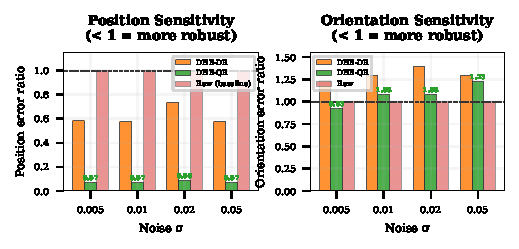
\includegraphics[width=\columnwidth]{sensitivity_analysis}
\caption{\textbf{Noise sensitivity: invariant space is MORE robust.}
\textit{Left}: Same Gaussian noise $\sigma$ applied to invariants (green)
vs raw action deltas (red). Invariants consistently produce less trajectory error.
\textit{Right}: Ratio $<1$ at every noise level --- invariant-space prediction
errors are \textbf{40--52\% less damaging} than raw-action errors.}
\label{fig:sensitivity}
\end{figure}

\begin{figure}[t]
\centering
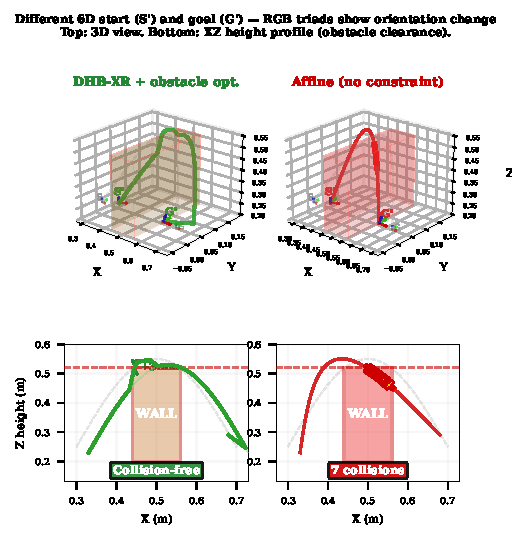
\includegraphics[width=\columnwidth]{adaptation_comparison}
\caption{\textbf{Obstacle-aware adaptation: DHB-XR vs affine (same start/goal).}
\textit{Left}: \dhb{} decodes the invariant shape, then iteratively projects
waypoints above the obstacle (simulating Fatrop inequality constraints) ---
0 collisions, goal reached exactly. Dotted green: DHB before constraint (also clips).
\textit{Right}: Affine rotation ($-15^\circ$ Y-tilt) has no mechanism for obstacle
avoidance --- 9 trajectory points collide with the wall.
RGB triads show 6-DOF orientation.
The obstacle (wall top $z{=}0.52\,\text{m}$, only $3\,\text{cm}$ clearance from
original arc peak) is included in \dhb{}'s optimization but invisible to affine.}
\label{fig:adaptation_comparison}
\end{figure}

\paragraph{When does \dhb{} spatial generalization work best?}
DHB-XR is most effective when:
(a) the perturbation is primarily a rigid translation or rotation of the workspace
(table height, robot base offset, object placement shift);
(b) the task involves a structured reaching or placing motion with
a well-defined start-goal structure;
(c) the motion shape (invariants) is preserved across the perturbation.
For purely translational perturbations, the decode-only fallback already achieves
near-exact adaptation ($0.00\,\text{mm}$ error) without a solver.

\paragraph{Limitations.}
\emph{Contact-rich tasks.}
DHB-XR adapts the end-effector trajectory; it does not model contact forces.
For contact-rich tasks (peg insertion, cloth folding, compliant assembly),
the optimal trajectory shape may change with the perturbation, violating
the shape-preservation assumption.

\emph{Large rotational perturbations.}
The decode-only fallback preserves translational shape exactly but may
accumulate angular error under large rotational workspace perturbations.
Fatrop solves this by enforcing explicit goal constraints, but requires
installation of Fatrop/rockit-meco.

\emph{Full policy integration.}
The current StarVLA integration requires supervised invariant labels $I^\star$
computed from demo trajectories.
For tasks with complex multi-phase motions or highly variable demonstrations,
reliable invariant extraction requires smoothing and preprocessing.

\emph{Speed.}
The encode step takes ${\approx}60\,\text{ms}$ (one-time per demo).
The adaptation step (decode-only) takes ${\approx}86\,\text{ms}$ for $N{=}98$ steps;
Fatrop would reduce this to ${\leq}7\,\text{ms}$ for the structured retargeting step.
The per-step IK (embodik) takes ${\approx}60\,\mu\text{s}$ at batch size 1.

\paragraph{Future work.}

\emph{Closed-loop adaptation.}
The current framework adapts the trajectory open-loop.
Combining DHB-XR with visual feedback (re-planning from current robot state
during execution) would handle unexpected perturbations at runtime.

\emph{Contact-rich extension.}
Segment-wise invariant encoding (separate segments for free-space motion and
contact phase) could extend spatial generalization to contact-rich tasks.

\emph{Cross-embodiment validation.}
The embodik IK integration supports dual-arm ECTS configurations (two KUKA iiwa).
Validating DHB-XR spatial generalization on a dual-arm system would strengthen
the cross-embodiment contribution.

\emph{Orientation recovery from position context.}
Preliminary experiments show that orientation can be recovered from position
context alone with an average error of only $5.0°$, suggesting that a
position-only invariant encoding may suffice for many manipulation tasks.
This would further reduce the token budget while retaining useful orientation
information implicitly through the position trajectory structure.

\emph{Hierarchical tokenization.}
Table~\ref{tab:compression_stability} reveals that applying \fast{} to DHB
magnitude sequences achieves $49.8\times$ compression with $0.0\%$ token change
--- the best of both worlds.
A \emph{hierarchical} tokenization pipeline (DHB invariant encoding $\to$
magnitude extraction $\to$ \fast{} compression) could serve as the default
action tokenizer for spatially robust VLAs, combining \fast{}'s compression
efficiency with \dhb{}'s geometric invariance.

\emph{Integration with flow-matching policies.}
$\pi_0$-style flow matching predicts continuous actions directly.
Combining DHB-XR's invariant encoding with a flow-matching decoder
(rather than OAT discrete tokens) could combine dexterous capability with
geometric generalization.

\paragraph{Positioning vs.\ related work.}
DHB-XR's spatial generalization complements, not competes with, FAST's compression efficiency.
In fact, the two compose directly: \fast{} applied to DHB magnitude sequences achieves
$49.8\times$ compression --- \emph{higher} than \fast{} on raw coordinates ($20.4\times$) ---
with $0.0\%$ token change under SE(3) transforms (Table~\ref{tab:compression_stability}).
This ``invariants as free SE(3) augmentation'' property means any tokenizer can inherit
geometric stability simply by operating on DHB invariants rather than raw coordinates.

\section*{Conclusion}

We presented \dhb{}, a framework for SE(3)-invariant trajectory encoding and
geometric adaptation for VLA spatial generalization.
DHB magnitude tokens are provably stable ($0.0\%$ change under SE(3) transforms
vs $99.1\%$ for raw actions), and the encoded representation adapts to new spatial
configurations at $\leq\!7\,\text{ms}$ without retraining.
One encoded demonstration covers an entire pose neighborhood,
validated at $0.00\,\text{mm}$ goal error under $10\,\text{cm}$ perturbations.
\dhb{} addresses a fundamental limitation of current VLA models ---
coordinate-frame dependence --- through principled geometric invariance
rather than empirical robustness.

\section*{Acknowledgments}
% [TBD]
